\documentclass[a4paper,10pt]{article}

% include headers and preamble for reoport
% file: includes-report.tex
% -----------------------------------------------------------------------------
% includes for studies report
% -----------------------------------------------------------------------------

\usepackage{amsmath}
\usepackage{setspace}
\usepackage[top=1.2in, bottom=1.2in]{geometry}
\usepackage[x11names]{xcolor}

\usepackage{float} % to force placement of images etc.

\usepackage{graphicx}
\usepackage[utf8]{inputenc}
\usepackage{siunitx}

% // -- for different section heading color --
\usepackage{sectsty}
\usepackage{xcolor}
% \chapterfont{\color{blue}}  % sets colour of chapters
% \definecolor{MyBlue}{rgb}{0.78,0.9,1} % rgb color code
% \definecolor{DarkBlue}{HTML}{002f4c} % HTML HEX color code
\definecolor{DarkBlue}{RGB}{0,47,76} % RGB color code
\sectionfont{\color{DarkBlue}}  % sets colour of sections
\subsectionfont{\color{DarkBlue}}  % sets colour of sections

\usepackage{float}


%\usepackage{multirow}
%\usepackage{pgfplots}
\usepackage{subcaption}

% // -- for source code listings --
\usepackage{color}
\definecolor{OliveGreen}{RGB}{0,128,0}
\usepackage{listings}
\usepackage{caption}
\DeclareCaptionFont{white}{\color{white}}
\DeclareCaptionFormat{listing}{\colorbox{gray}{\parbox{\textwidth}{#1#2#3}}}
\captionsetup[lstlisting]{format=listing,labelfont=white,textfont=white}


\lstdefinestyle{cStyle}{language=C}
\lstset{
language=C,
%basicstyle=\small\ttfamily,
basicstyle=\small\ttfamily,
keywordstyle=\color{blue}\ttfamily,
stringstyle=\color{red}\ttfamily,
commentstyle=\color{magenta}\ttfamily,
morecomment=[l][\color{magenta}]{\#},
numbers=left,
numberstyle=\tiny,
% frame=tb,
columns=fullflexible,
showstringspaces=false,
tabsize=2
}
\usepackage{matlab-prettifier}
\lstdefinestyle{matlabStyle}{language=matlab}
\lstset{
%style=Matlab-editor,
language=matlab,
%basicstyle=\small\ttfamily,
basicstyle=\small\ttfamily,
keywordstyle=\color{blue}\ttfamily,
stringstyle=\color{red}\ttfamily,
commentstyle=\color{OliveGreen}\ttfamily,
morecomment=[l][\color{OliveGreen}]{\#},
numbers=left,
numberstyle=\tiny,
% frame=tb,
columns=fullflexible,
showstringspaces=false,
tabsize=2
}
\lstdefinestyle{vhdlStyle}{language=vhdl}
\lstset{
language=vhdl,
%basicstyle=\small\ttfamily,
basicstyle=\small\ttfamily,
keywordstyle=\color{blue}\ttfamily,
stringstyle=\color{red}\ttfamily,
commentstyle=\color{magenta}\ttfamily,
morecomment=[l][\color{magenta}]{\#},
numbers=left,
numberstyle=\tiny,
% frame=tb,
columns=fullflexible,
showstringspaces=false,
tabsize=2
}

% bibliography (Literaturverzeinis)
\usepackage[round]{natbib}
\bibliographystyle{alphadin} % set format

% // -- source code listings --


\title{Bachelorprojekt}
\date{2017-MM-DD}
\author{AUTHOR}

\begin{document}

% Titlepage for HAW lab report
% \begin{titlepage}
% \definecolor{blue(ncs)}{rgb}{0.0, 0.53, 0.74}
% \begin{figure}[h!]
% 	\begin{flushright}
% 	\begin{spacing}{1.5}
% 	
\includegraphics[width=.5\linewidth]{images/hawlogo.png}
%   \label{fig:hawlogo}\\
% 	\small Fakultät Technik und Informatik\\
% 	\small Department Informations- und Elektrotechnik
% 	\end{spacing}
% 	\end{flushright}
% \end{figure}
% \textbf{\large Labor für XXX}
% \begin{center}\noindent\textcolor{blue(ncs)}{\rule{13.5cm}{0.5mm}}\end{center}
% \begin{spacing}{4.5}
% \textbf{\huge Bachelorprojekt}
% \end{spacing}
% \textbf{\large\indent Blabla irgendwas mit autonomen Fahren}
% \begin{center}\noindent\textcolor{blue(ncs)}{\rule{13.5cm}{0.5mm}}\end{center}
% \begin{spacing}{1.15}
% \vspace*{\fill}
% \noindent
% \textnormal{\\
% 	Prof. Dr.-Ing. Marc Hensel \\
% 	\textbf{Projektgruppe:} Fabian Huber, Enzo Morino, Markus Trockel \\
% 	\textbf{Abgabe:} DD.MM.2017 \\
% }
% \end{spacing}
% \end{titlepage}
% --- end of titlepage ---

  \pagenumbering{gobble}
  \newpage

  \tableofcontents
  \newpage

  \pagenumbering{arabic}

  \section{1. Abschnitt}
  % cite from bibtex file
  Blabla filltext foobar \cite{wikipedia:foobar}... \\
  
  %Aufbau ist in Fig. \ref{fig:aufbau}\cite{AUFGABENSTELLUNG:1} zu sehen.\\

    %% insert code listing from file
    % \lstinputlisting[style=cStyle,label=python-01,caption=Python-Code]{filename.py}

    %% insert code listing in line
    \lstinline{int voyager = 0;}

    \begin{lstlisting}[style=pythonStyle,label=python-02,caption=Python-Code]
    while True:
        if (sonic.getDistance() < 60):
            print "Proximity alert!"
            # act.sendCommand(act.STOP)
            # sleep(5)
            # act.sendCommand(act.FWD)
        else:
            command = cam.getCommand()
            # send to motor control
            message = act.sendCommand(command)
            if message == act.ERROR:
                # raise Exception('modAct returned ERROR')
                print ('modAct Error: ' + str(message))
                cam.cv.waitKey(0)
            # print ("Command received: " + outputCommand(command) + ' (Code: ' + str(command) + ')')
            outputVideo(command)
    \end{lstlisting}
  % \\
 
    %% image
    \begin{minipage}{\columnwidth}
      \makeatletter
      \def\@captype{figure}
      \makeatother
      \centering
      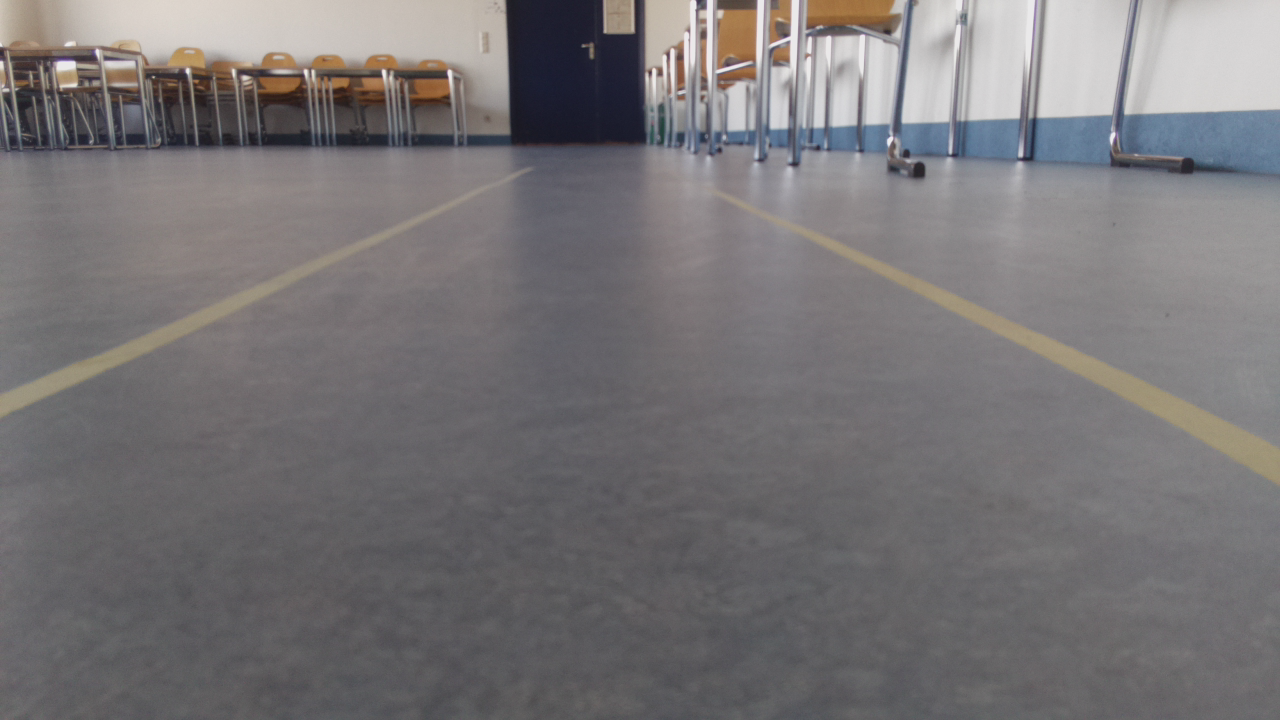
\includegraphics[width=0.8\linewidth]{images/image.png}
      \caption{Text underneath the image}
      \label{fig:image-01}
    \end{minipage}
  %\\

  %% table
    \begin{minipage}{\columnwidth}
      \makeatletter
      \def\@captype{table}
      \makeatother
      \centering
      %\rowcolors{1}{grey}{white}
      \begin{tabular}{ l | c }
      % \multicolumn{2}{|c}{Frame \#} & \multicolumn{4}{|c}{LCD 0/3} &
      a & b \\ \hline \hline
      1 & 2 \\
      \end{tabular}
      \caption{Messergebnisse}
      \label{tab:122}
    \end{minipage}
  % \\

  %% listing
  \begin{itemize}
  \item{a)} erstes Stichwort
  \item zweites Stichwort
  \end{itemize}
  % \\

  \section{2. Abschnitt}
    Blabla filltext ... \\

	\bibliography{hawey-documentation}
  \bibliographystyle{ieeetr}

\end{document}
